\Chapter{Koncepció}

A játékot röviden, nagyjából összefoglaló folyamatábra amelyben a közelharc szekvenciát részleteztük egy új folyamatábrában a láthatóság kedvéért. Combat folyamatábra (\ref{fig:combat}. ábra).

\begin{figure}[h]
	\centering
	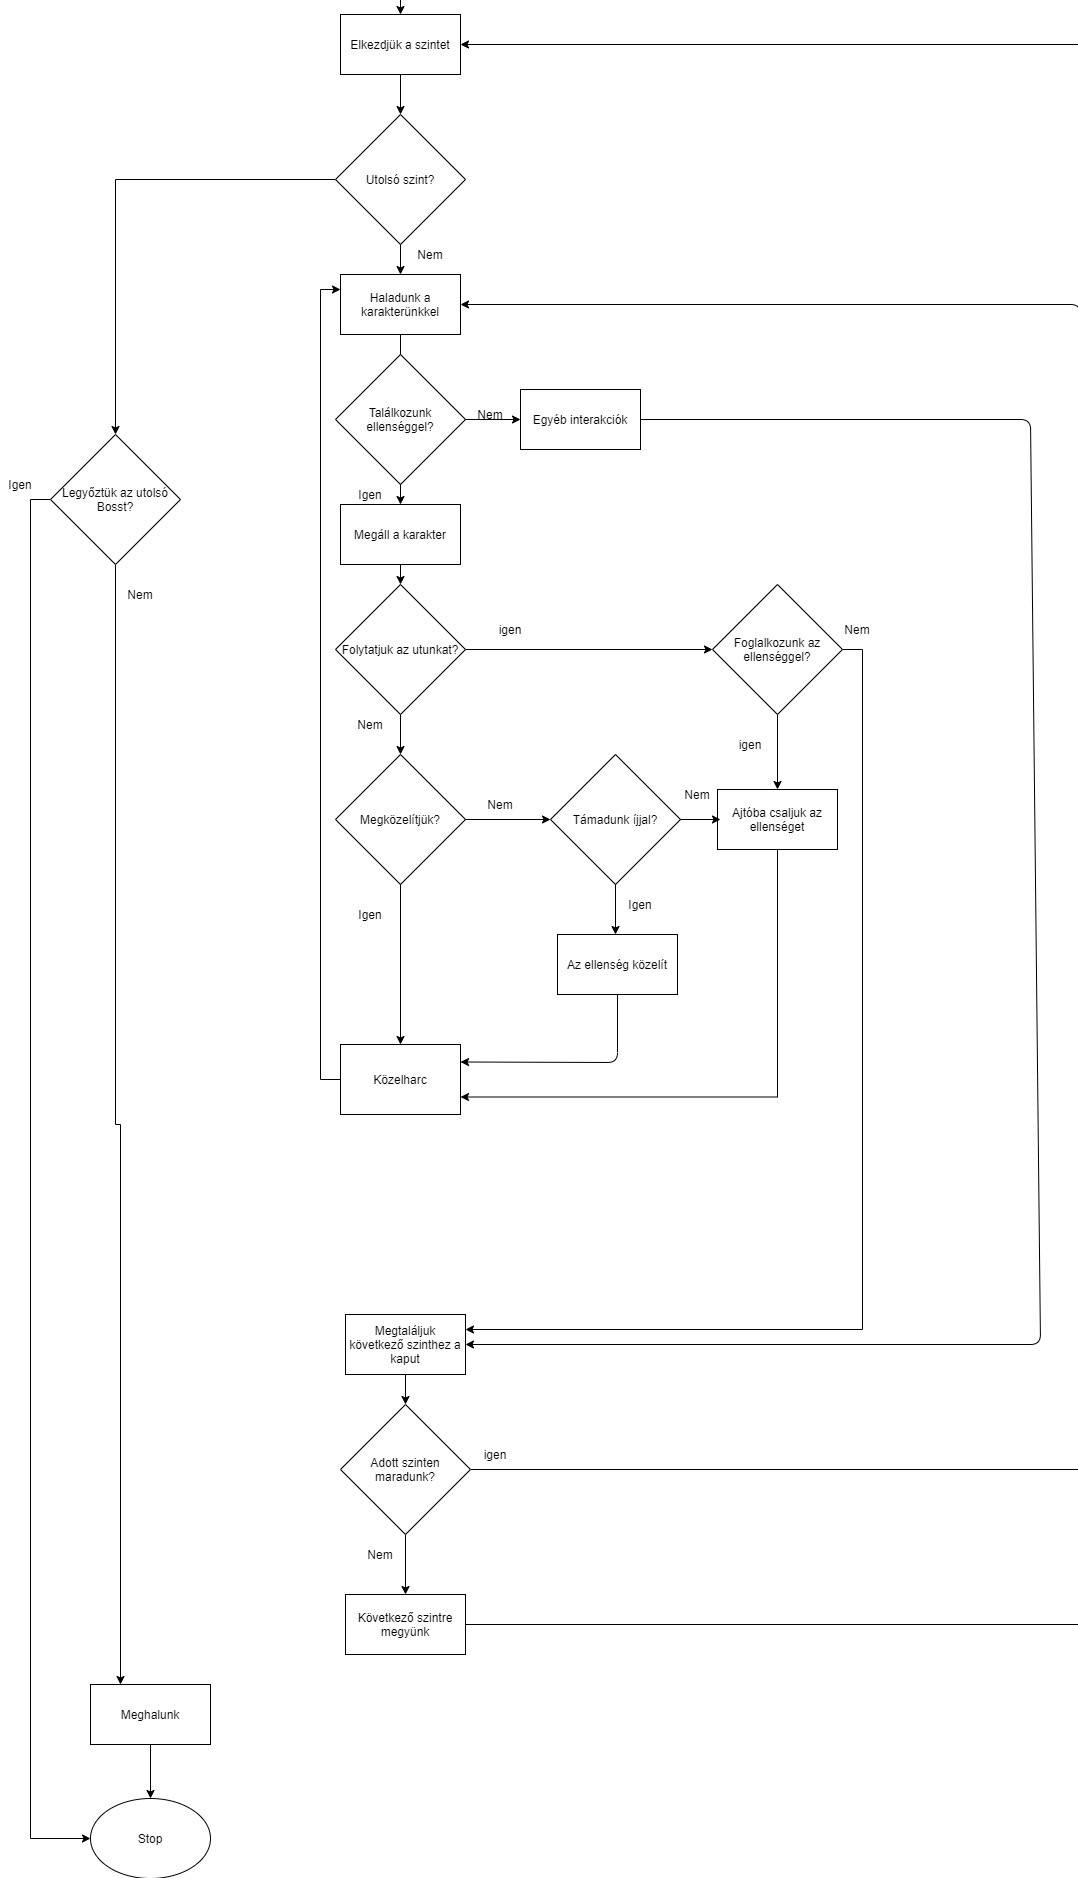
\includegraphics[width=\textwidth]{images/image1.png}
	\caption{Combat folyamatábra}
	\label{fig:combat}
\end{figure}

\Section{Menü}

A játék indításakor vagy megállításakor felugró ablak.
Start/Continue:
A játék indításakor a menüben a start-ot látjuk, ha a játékot állítjuk meg, akkor a menüben a continue-t látjuk.
Ezen menüpont kiválasztásával kezdhetjük a játékmenetünket vagy folytathatjuk azt.
Save:
Ez a menüpont nem jelenik meg a játék indításakor csak akkor, hogyha játékmenetet állítunk meg.
Ezen menüpont kiválasztásával menthetjük a jelenlegi játékmenetünket.
Load:
Ezen menüpont mindig jelen van a menüben, elérhető a játék indításakor és megállításakor is.
Ezen menüpont kiválasztásával tölthetjük be az általunk lementett mentéseket.
Options:
Ezen menüpont mindig jelen van a menüben, elérhető a játék indításakor és megállításakor is.
Ezen menüpont kiválasztásával egy új ablakra irányít át minket.
Itt lehetőségünk van hangbeállítások személyre szabására, mint például a zene és a játékbeli hangok. (Több csúszka segítségével)
Lehetőségünk van fényerő beállításokra is, mint például a Gamma állítására. (Egy csúszka segítségével)
Nyelvi beállítások a menüre vonatkozóan. (Legördülő fülből kiválasztva)
Vér ki/bekacsolása játék közben. (Egy ki/bepipálható rublika)
Végezetül egy visszagomb ami visszairányít minket a menübe.
Rankings(history):
A főmenüben található rákattintásakor felugrik egy ablak amiben összes régebbi karakterünk alapstatisztikáit kilistázza.
Badges(achievements):
Szintén a főmenüből elérhető, megnyitásakor a játékban szerzett cselekedeteink után kapunk jelvényeket.
Log out:
Kiléptet minket a jelenlegi fiókunkból, visszairányítva a bejelentkezési ablakhoz.
A log-out a menüben mindig szerepel.
Main menu:
Ez a gomb akkor szerepel a menüben hogyha egy játékmenet megállításával kerülünk a menübe.
Ez befejezi a jelenlegi játékmenetünket és visszaírányít minket a főmenübe.

\begin{figure}[h]
	\centering
	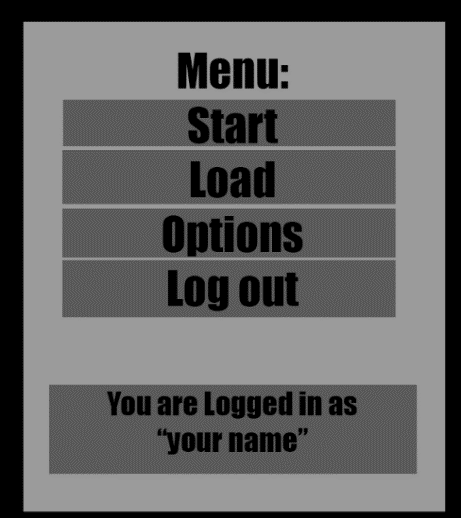
\includegraphics[scale=1]{images/image2.png}
	\caption{Főmenü}
	\label{fig:image2}
\end{figure}

\begin{figure}[h]
	\centering
	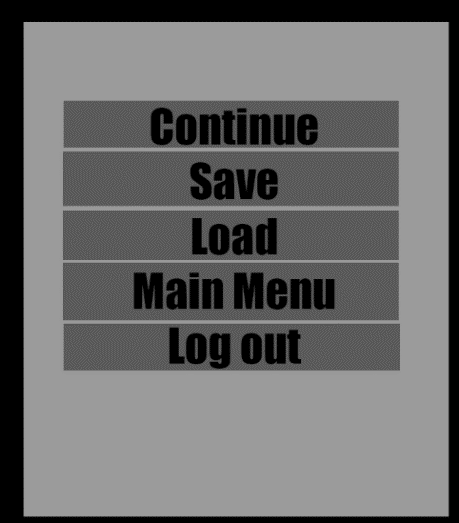
\includegraphics[scale=1]{images/image3.png}
	\caption{Játékbeli menü}
	\label{fig:image3}
\end{figure}

\begin{figure}[h]
	\centering
	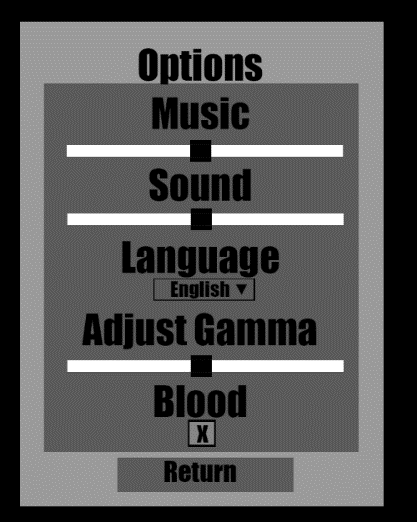
\includegraphics[scale=1]{images/image4.png}
	\caption{Options}
	\label{fig:image4}
\end{figure}

Ahol a Fekete háttér, az a megállított játék képe lenne elhomályosítva.
Ha még nem kezdtünk bele egy játékmenetbe, akkor pedig általunk megadott játékmenet képernyőmentése lenne a háttérben elhomályosítva.

\Section{Map}

Általunk előre definiált szobatípusokból generált, de szinthez kötötten meg van adva a minimum generálható szoba és a maximum generálható szoba száma.
Szinthez kötötten adott típusú és mennyiségű entity.
Minden mapnak van kezdő és végpontja, amely a következő mapra visz minket.
A szobákat változó hosszágú folyosók kötik össze.
Szobatípusok:
Ezek többnyire mechanikai és grafikai tematikájukban különböznek.
Alap:
Ez a szobatípus nem tartalmaz speciális platformokat.Tetszőleges alakú de páros számú fallal rendelkezik(falak csak X vagy Y tengellyel lehetnek párhuzamosak).
Vizes mocsaras környezet:
Ez a szobatípus tartalmaz speciális platformokat mint például mocsár(lelassítja a mozgást alapesetben), víz(bizonyos ellenségek vízben jobban mozognak, mint mi alapesetben).
Tetszőleges alakú de páros számú fallal rendelkezik(falak csak X vagy Y tengellyel lehetnek párhuzamosak).
Kovácsműhely:
Ebben a szobában nincsenek ellenfelek, tárgyak és ládák. Itt tudunk karakterünkkel különböző itemeket készíteni/fejleszteni. A platform kövezett, fegyverek és páncélok díszítik a falakat. Ezek a szobáknak csak egy ajtajuk van. Tartalmaz egy interaktív térbeli objektumot, amely segítségével tehetjük meg a fent említett tevékenységeket.
Főzetkészítő szoba: 
Ebben a szobában nincsenek ellenfelek, tárgyak és ládák. A platform fából készített, ahogyan a falak is. Ezeknek a szobáknak csak egy ajtajuk van. Tartalmaz egy interaktív térbeli objektumot, ami segítségével készíthetünk főzeteket.
Csapdaszobák:
Általában valamilyen ládát tartalmaznak a belsejükben.
Különböző dizájnú platformok lehetnek, de nem speciálisak. De tartalmazhatnak nagy valószínűséggel csapdákat.

A csapdák gyakran nem láthatóak, a játékos a keresés akcióval felderítheti a körülötte lévő platformokon rejtve hagyott csapdákat.
Minden csapdának más grafikus megjelenése van.
A csapdák akkor aktiválódnak, ha a platformra lépünk vagy a játékos által egy item kerül eldobásra az adott platformra.
A csapdák rálépésekor különböző főzet effekteket rakhatnak ránk, vagy egyéb speciális akciókat hajtanak végre(hangcsapda, amely a körülöttünk lévő szobákból hozzánk hívja az ellenfeleket).
A csapdák aktiválása elkerülhető lebegő effekt használatával amely vagy főzet vagy item vagy speciális térelemektől szerezhetőek. Ezek a szobáknak csak egy ajtajuk van. Általában itemet vagy ládát tartalmaznak.
Titkos szobák:
Ezeket a szobákat titkos falak vagy zárt ajtók mögött találhatjuk, általában itemet vagy ládát tartalmaz, számuk limitált 5 szintenként 1 ilyen szoba generálódhat le. Pókhálós környezet, néhol hiányzó platform. Ezek a szobáknak csak egy ajtajuk van.
Mini boss szobák:
Egyedül a mini boss található meg bennük mint ellenség, ha megtámadjuk akkor viszonozza a támadást. Ez egy egyedi ellenségtípus. Szobán belül nincsenek itemek és térbeli elemek.
A mini-boss addig alszik amíg nem támadja meg a játékos.
Boss szobák:
A boss szobák csak a boss mapján találhatóak meg, változó nagyságúak lehetnek.
Minden bossnak különböző szobái vannak különböző objektumokkal.
A boss szintet nem léphetik át amíg meg nem ölték.
Egyéb:
A szobák formáit akkor láthatjuk, ha nem tartózkodunk benne, ha már voltunk benne előzőlegesen vagy ha felderítettük főzettel. Ekkor nem látjuk, hogy milyen változók vannak benne. (Itemek és Entityk)

\Section{Szint}

Karakter alapstatisztikái:
\begin{itemize}
    \item HP:20
    \item Erő:4
    \item Intelligencia:3
    \item Ügyesség:3
\end{itemize}

Megölt ellenség után kapunk tapasztalatipontot az alapján, hogy milyen tipusú az ellenség.

Valahányszor amikor karakterünk szintet lép, kapunk 1 pontot.

A második szint eléréséhez 20 tapasztalatipont minden következő szinthez +5 tapasztalatipont elérése szükséges az előző szinthez képest.

A karakter ablakon belül 4 lehetőség van, amelyek közül választhatunk mit fejleszthetjük tovább:
\begin{itemize}
    \item Vitalitás: Megnöveli a maximális életerőnket.
    \item Erő: Erősíti a fizikai támadásokat.
    \item Intelligencia: Erősíti a mágikus támadásokat.
    \item Ügyesség: Erősíti a Íjjal való támadásainkat.
\end{itemize}

Minden következő szint több entity megölését igényli.
Minden vitalitáspont +2 életerőt ad.

% TODO: Az ellenség és az entity ugyanazt jelentené? (Ezt pontosítani kellene.)

Minden erőpont +2 növeli a fizikai támadásainkat.
Minden intelligenciapont +1-el növeli a mágikus támadásainkat.

Minden ügyességpont +1-el növeli a íjjal való támadásainkat.

Minden stat 5-ször fejleszthető.

\Section{Combat}

A combat akkor kezdődik, ha ellenséggel találkozunk, és az észrevesz minket, ha nem, akkor lehetséges a rajtaütés.

\SubSection{Melee combat}

Közvetlen közelünkben (1 blokknyi távolságra, vagy vízszintesen, vagy függőlegesen).
Kezdeményezéstől függően dől el ki fogja elkezdeni a harcot, innentől kezdve a két fél felváltva hajtanak végre 1 támadást amivel párhuzamosan történik a sebzés illetve a kitérés, (kitérés: \%-os eséllyel elháríthatunk egy támadást ami után 0 sebzést szenved el az adott harcos) (sebzés:A harcost érő találat és a felszereléséből adott összesített védelem különbségből adódik.A számítás után kapott összeget levonjuk a harcos aktuális életerejéből) ez addig folytatódik amíg valamelyik fél életereje el nem éri a 0-át.Ezután a vesztes fél eldobja nála lévő tárgyait és a combatnak vége.

Ha a menekülést választjuk és sikerült továbblépnünk a következő szintre anélkül hogy az ellenfél elkapott volna, az üldöző nem tud tovább lépni a következő szintre.

\SubSection{Ranged combat}

Adott távolságon belül, adott támadással.
Karakterünk alapfelszerelésében található 10db nyilvessző, inventory helyén kívül a jobb alsó sarokban kapott egy saját gombot aminek rákattintásával 1db nyílvesszőt eldobhatunk arra amerre célzunk az így okozott sebzés nem lehet több 2-nél alapesetben.

% TODO: A grafikus megjelenítést és a mögötte lévő modellt nem érdemes keverni. Tipikusan először a modellt, majd annak reprezentációját érdemes bemutatni.

\begin{figure}[h]
	\centering
	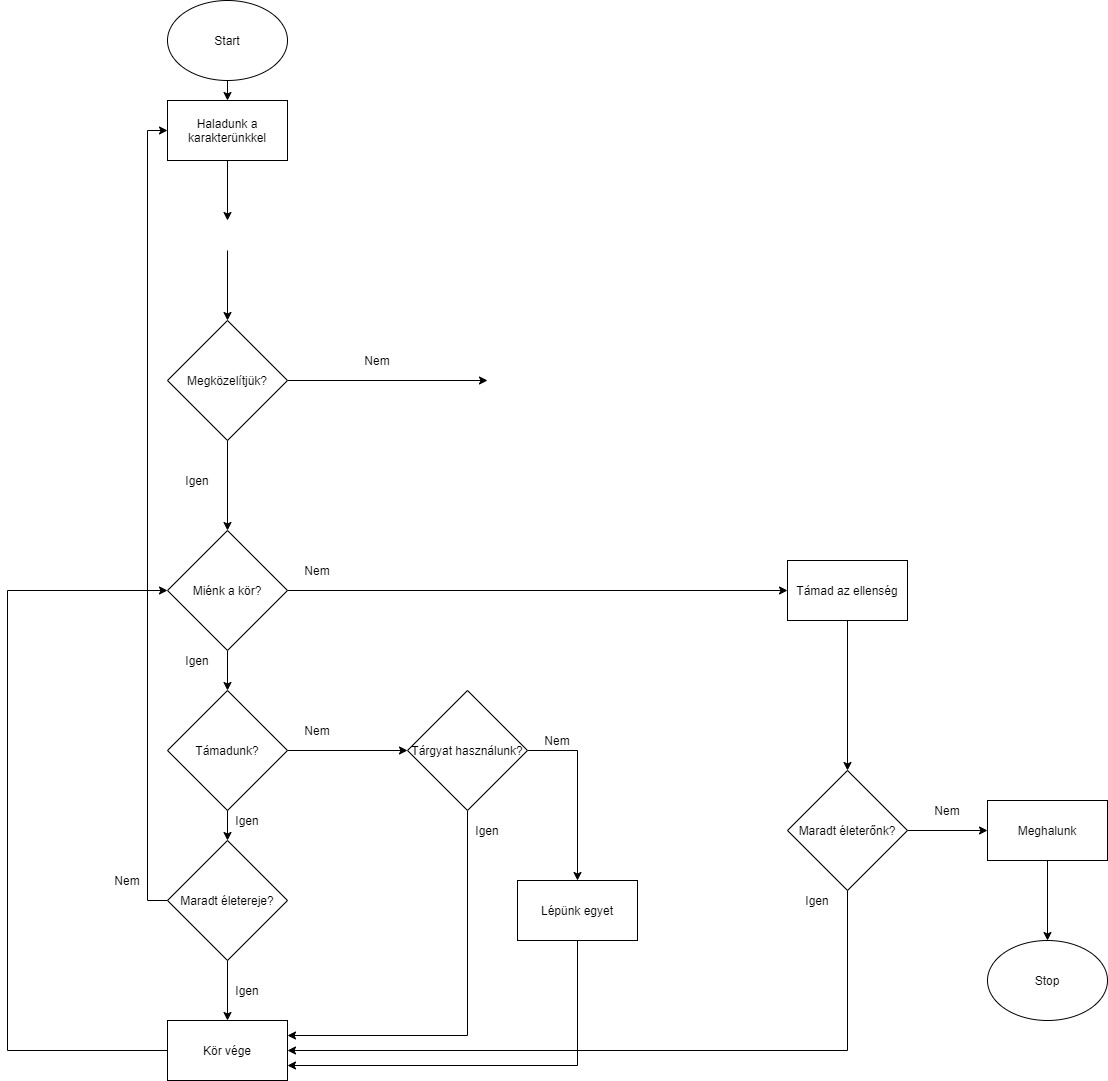
\includegraphics[width=\textwidth]{images/image5.png}
	\caption{Combat folyamatábra}
	\label{fig:combat2}
\end{figure}

\Section{Entity}

Egy platformon csak egy darab entity lehet, nem lehet rajtuk átmenni.

\noindent No. 1. Entity:
\begin{itemize}
    \item Körönként 1 lépést tesz meg.
    \item Körönként 1 támadást hajt végre.
    \item Nagyobb kitérés.
    \item Ajtóban sebezhetőek az első támadásig.
    \item Halálukkor 5 tapasztalati pontot adnak.
\end{itemize}

\noindent No. 2. Entity:
\begin{itemize}
    \item Körönként 1 lépést tesz meg.
    \item Körönként 1 támadást hajt végre.
    \item Halálukkor 3 tapasztalati pontot adnak.
\end{itemize}

\noindent No. 3. Entity:
\begin{itemize}
    \item Körönként 3 lépést tesz meg.
    \item Körönként 3 támadást hajt végre.
    \item Halálukkor 4 tapasztalati pontot adnak.
\end{itemize}

\noindent No. 4. Entity:
\begin{itemize}
    \item Körönként 1 lépést tesz meg.
    \item Körönként 3 támadást hajt végre.
    \item Halálukkor 4 tapasztalati pontot adnak.
    \item Képes ranged attack-ok végrehajtására 3 blocknyi távolságból.
\end{itemize}

\noindent Egyéb:
\begin{itemize}
    \item Az Entytik elkerülik a rejtett csapdákat.
    \item Az Entytik 80\%-a alvó állapotba kerül be a szobák egyikébe és úgy is marad amíg meg nem közelíti a játékos az adott szobát.
    \item A többi nem alvó szabadon mozog, valahányszor mi is kört igénylő cselekvést hajtunk végbe.
\end{itemize}

\Section{Térbeli objektumok}

A térbeli objektumokra karakterünk nem képes rálépni, nem lát át rajtuk.
\begin{itemize}
\item
Ajtók: Karakterünk vagy egyéb entity-k az ajtó poziciójára lépnek akkor az ajtó kinyílik ha nem kulccsal zárt.
\item
Zárt ajtók: Rákattintunk és a karakterünk a közvetlen közelébe megy és van nálunk hozzá megfelelő kulcsunk akkor a karakterünk egy körért cserébe eltávolítja a zárt az ajtóról, ezek után sima ajtóként funkcionál.
\item
Kovácsműhely: Rákattintunk és a karakterünk a közvetlen közelébe megy, ha odaértünk akkor karakterünk interaktál vele és megnyílik egy felugró ablak. A szerzett alapanyagok segítségével tudjuk továbbfejleszteni a már meglévő felszereléseinket. Egy körbe kerül.
\item
Félkarú rabló: Rákattintunk és a karakterünk a közvetlen közelébe megy, ha odaértünk akkor karakterünk interaktál vele és megnyílik egy felugró ablak. Az általunk birtokolt aranyért cserébe esélyünk van játszani a félkarú rablón ami egy körbe kerül.A félkarú rabló nem mindig ad vissza tárgyat csak ha nyerünk vele.A nyeremény az az item amit 3-szor egymás után kipörget a játékos, egy játékon belül.
\item
Főzetfőző állomány: Rákattintunk és a karakterünk a közvetlen közelébe megy, ha odaértünk akkor karakterünk interaktál vele és megnyílik egy felugró ablak. Az általunk birtokolt növényi alapanyagok használatával véletlenszerű fözetet készíthetünk, legalább 3 alapanyag szükséges hozzá.
\item
Ércek: Rákattintunk és a karakterünk a közvetlen közelébe megy, ha odaértünk akkor karakterünk egy körért cserébe eltünteti a közvetlen közelünkben lévő ércet és kapunk egy alapanyagot.
\item
Láda: Rákattintunk és a karakterünk a közvetlen közelébe megy, ha odaértünk akkor karakterünk interaktál vele. A láda ezekután eltünik és egy tárgyat hagy hátra.
\item
Zárt láda: Rákattintunk és a karakterünk a közvetlen közelébe megy, ha odaértünk akkor karakterünk interaktál vele ha van hozzá megfelelő kulcs és a zárt láda átalakul sima ládává.
\item
Lépcsők: Rákattintunk és a karakterünk a közvetlen közelébe megy, ha odaértünk akkor karakterünk a következő szintre lép.
\end{itemize}

\Section{Loot}

Az ellenfelek halál esetén \%-os eséllyel hagynak hátra maguk után valamilyen itemet.

A tárgyak amelyeket nem veszünk fel a játék végéig ott maradnak.

Minden entity más itemet hagyhat maga után.
Bizonyos térbeli elemek is adhatnak különböző itemeket.

Bizonyos ládák illetve ajtók kulcsot, igényelhetnek.
Bármely ellenfél dobhat \%-os eséllyel legalább 20 legfeljebb 70 aranyat, amit félkarú rablóknál lehet elkölteni felszerelések fejlesztésére.

Néhány alap szoba,folyosó platformjainak felét fű borítja amelynek letaposásából \%-os eséllyel kaphatunk magvakat amiket el lehet ültetni ezzel csapdát állítva ellenfeleknek illetve szemgolyókat amik 1 életerőt gyógyítanak.

Alapfelszerelésen kívül minden felszerelés amit lootolunk számunkra ismeretlen felvételükkor 10 körig nem lehet levenni őket és a körök lejárta után pozitív vagy negatív effektet adnak.

Szemgolyókon kívül minden item amit lootolhatunk hatásuk számunkra ismeretlen első használatkor, a játék előrehaladtával ismerjük meg különböző tekercsek illetve főzetek effektjeit,a már egyszer használt itemek effektjeit karakterünk ismeri.

\Section{Itemek}

Az itemek a földről úgy vehetőek fel, hogy karakterünk arra a blokkra lép ahol az item található, ekkor megjelenik egy gomb amely rákattintásakor felveszi az itemet hogyha van hely az inventorynkban.

Az inventory mérete fix legyen 20 egység pl.: 4 egység széles 5 egység magas elosztásban.
Az inventoryból minden item egyetlen egy egységet igényel tárolásra.

Leltárban fix helye van az aranynak a jobb alsó sarokban.

Minden tárgyból bármekkora mennyiséget lehet tárolni.
Egyes objectek nem kerülnek az inventory-ba ennek oka hogy hatásukat kifejtik felvételükkör.(szemgolyók)

Entityk vagy térbeli elemek adják.
különböző felhasználási lehetőségekkel.
Fegyverek, Armorok.

Bizonyos stat növelők (Főzetek).
Minden tárgynak, amelyet Entitykből vagy térbeli objektumokból szerezhetőek meg, nem fix esélyű tárgyak.

\SubSection{Kulcsok}

Minden mapon annyi kulcs spawnol, véletlenszerűen a szobák egyikébe amennyi kulcs\-csal zárt ajtó generálódott a mapra.

Különleges Kulcsok:
Máshogy néznek ki grafikailag, mint a sima kulcs és külön vannak tárolva tőlük. Ezek a kulcsok a zárt ládák kinyitására használhatóak.

Ha a mapon van zárt láda, mindig 2 van közel egymáshoz. És a mapra mindig csak 1 kulcs kerül hozzá.

\SubSection{Alapanyagok}

Bizonyos felszerélesek fejlesztéséhez bizonyos alapanyagok szükségesek, ezeket megszerezhetjük ellenségektől vagy térbeli objektumokkal.
Ilyen térbeli objektum például egy érc, vagy egy növény.

A főzetek készítéséhez is szükségünk van alapanyagokra, ezeket szintén Entityk is dobhatják, de beszerezhetjük őket növényekből is.

\SubSection{Magvak}

Füves platformok letaposásából kaphatunk \%-os eséllyel.
Mindenfajta magvat el lehet dobni ilyenkor a magból kikelt növény hatása a helyétől körben 1 block távolságban fejti ki hatását 3 körig.

Magvak típusai:

borotva: Eltiprásakor(rálépésekor) aktiválódik a hatása, ami az elültetés helyétől körben 1 platformnyi távolságra 3-at sebez az aktiválás utáni első körben.

gyógyító: Eltiprásakor(rálépésekor) aktiválódik a hatása, ami elültetés helyétől körben 1 platformnyi távolságra 3-at gyógyít az aktiválás utáni első körben.

mérgező: Eltiprásakor(rálépésekor) aktiválódik a hatása, ami elültetés helyétől körben 1 platformnyi távolságra méreg effektet rak az egységre amely 2 körön keresztül sebez 2-őt.

\SubSection{Főzetek}

Játékban talált alapanyagokat összefőzhetjük egy adott főzőállomásnál , amely egy véletlenszerű hatású főzetet ad vissza nekünk.
Továbbá szimplán találhatunk szobákban ismeretlen főzeteket.
Minden főzetet el lehet dobni vagy meglehet inni, ilyenkor a becsapódás helyétől körben 1 block-nyira hat.

Főzetek típusai:
\begin{itemize}
\item Gyógyítás: A jelenlegi HP-nk 80\%-át visszatölti használatkor.
\item Mérgezés: Megmérgez minket, amely körönként 3 sebzést okoz, 3körig. Ellenségre is lehet dobni.
\item Altató: Elaltat minket 3körig, ellenségre is alkalmazható.
\item Azonnali sebzés: Használatkor azonnal sebez 30\%-ot a maximum HP-ból. Ellenségre is alkalmazható.
\item Teleport: Használatkor elteleportálja a karakterünket véletlenszerű helyre a mapon belül, eldobáskor maximum 3 entityt, saját magunkat beleszámolva telepíthet el, több különböző helyre.
\item Felderítő: Minden szobát úgy látunk, mintha már lettünk volna ott előzőleg. Véglegesen.
\item Lebegés: Csapdákat, vizes területeket, kerülhetünk el használatkor.10 körig tart a hatása.
\end{itemize}

\Section{Idő}

A szobán belülre kattintva odamegy a karakter ahova kattintunk, ha nem fedezz fel új ellenséget, ha mégis akkor megáll.

Az ellenfeleknek annyi akciója van amennyi akciót elvégeztünk a karaktereinkkel és velünk párhuzamosan cselekednek.

Az idő csak akkor telik amikor karakterünk végrehajt valamilyen akciót.Akciónak számít a mozgás, keresés, támadás, védekezés, tárgy használata.

\Section{Kamera}

Legyen a fény forrása a karakter, az adott szobában, nagyságától függetlenül minden ki van világítva, hogyha nem akadályozza semmi a fény útját.
A szobákat mindig felülnézetben láthatjuk, ahol a kamera leköveti a karakter mozgását, úgy hogy mindig középen legyen az.
A bal egérgomb letartásával és egér mozgatásával tudjuk mozgatni a kamerát.

\begin{figure}[h]
	\centering
	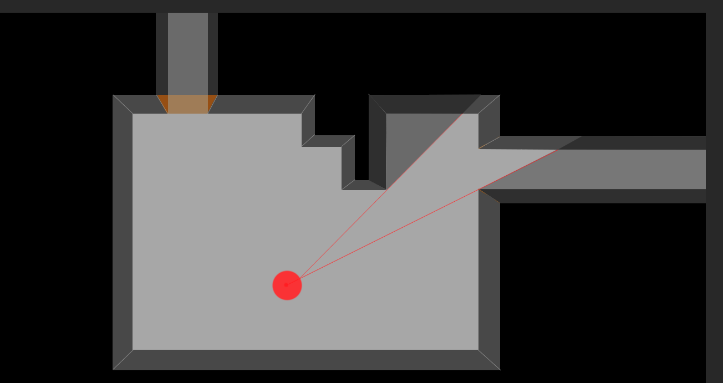
\includegraphics[scale=1]{images/image6.png}
	\caption{Kamera 1}
	\label{fig:camera1}
\end{figure}

\begin{figure}[h]
	\centering
	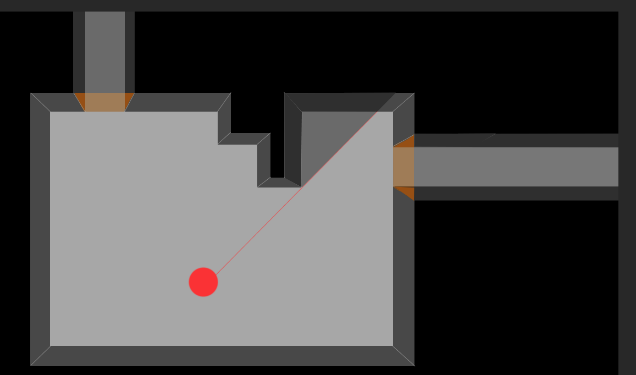
\includegraphics[scale=1]{images/image7.png}
	\caption{Kamera 2}
	\label{fig:camera2}
\end{figure}

A fenti képeken láthatunk egy szobát amelyben a karakterünk van (piros gömb), a fény arra terjed amerre a karakterünk forogna,ellátna.
Az ajtók ha nyitva vannak a fény továbbterjed a folyosóra.

\Section{Irányítás}

A kurzor használatával az adott területre kattintva halad oda a karakter.
Bizonyos helyezetekben megjelenő gombokra kattintva bizonyos tevékenységek lebonyolítása.
Egyéb menü/inventory megjelenítés bizonyos gombok segítségével(Esc,I, stb…)
A már általunk felfedezett területre kattintva karakterünk a lehető leggyorsabb útvonalat választja.

\Section{Az interface-n megjelenő gombok}

\SubSection{Tárgyfelvételi gomb}

\begin{itemize}
    \item prekondíció:A karakterünk egy tárgy helyén áll.
    általános müködés: Az egeret rávisszük a tárgyfelvételnek szánt gombra, és bal egérgombbal rákattintunk.
    \item alternatív esetek: Több item van egyhelyen, egyszerre csak egy itemet veszünk fel.
    \item postkondíció: Az item bekerült az inventorynkba.
    kivételes esetek: Nincs hely az inventoryban új tárgy felvételéhez.
\end{itemize}

\SubSection{Menü}

\begin{itemize}
    \item prekondíció: Játékmenetben vagyunk.
    általános működés: Az egeret rávisszük a menünek szánt gombra, és bal egérgombbal rákattintunk.
    \item alternatív esetek: Rossz ablak nyílik meg, nem pedig a menü, például az inventory.
    \item Postkondíció: Megnyílt a menü, válaszhatunk, hogy mit szeretnénk továbbá megnyitni. Az ablak jobb felső sarkában lévő X gombra kattintva visszatérünk a játékba.
    \item kivételes esetek: Nem nyílt meg a menü, bal egérgomb kattintásával.
\end{itemize}

\SubSection{Inventory}

\begin{itemize}
    \item prekondíció: Játékmenetben vagyunk.
    \item általános működés: : Az egeret rávisszük az inventorynak szánt gombra, és bal egérgombbal rákattintunk.
    \item Postkondíció: Megnyílt az inventory, válaszhatunk, hogy az inventoryban tárolt tárgyak közül melyikkel lépünk kapcsolatba. Az ablak jobb felső sarkában lévő X gombra kattintva visszatérünk a játékba.
    alternatív esetek: Rossz ablak nyílik meg, nem pedig az inventory, például a karakter.
    \item kivételes esetek: Nem nyílt meg az inventory, bal egérgomb kattintásával.
\end{itemize}

\SubSection{Íj}

\begin{itemize}
    \item prekondíció: Játékmenetben vagyunk.
    általános működés: : Az egeret rávisszük az íjnak szánt gombra, és bal egérgombbal rákattintunk.
    \item Postkondíció: Ha van ellenség adott távolságon belül, akkor megjelenik a legközelebbi ellenfelen egy célkereszt, amely után, ha rákattintunk, végbe megy a támadás. Ha nincs ellenség, nincs célkereszt.
    Lőttünk vagy abbahagytuk az adott cselekvést, a kurzor visszaalakul.
    \item alternatív esetek: Nincs nyíl a karakternél, nem megy végbe a támadás.
    \item kivételes esetek: Nem vált át íjra a karakter. Hiába kattintunk a gombra.
\end{itemize}

\SubSection{Súgó}

\begin{itemize}
    \item prekondíció: Játékmenetben vagyunk.
    általános működés: Az egeret rávisszük a súgónak szánt gombra, és bal egérgombbal rákattintunk.
    \item Postkondíció: : Ha a játékon belüli objectre kattintunk, akkor megjelenik egy felugró ablakban az adott object rövid leírása. Az ablak jobb felső sarkában lévő X gombra kattintva visszatérünk a játékba.
    \item alternatív esetek: Nem annak az objectnek jelenik meg a leírása, mint amire rákattintottunk.
    \item kivételes esetek: Nincsen elérhető információ az adott objectről.
\end{itemize}

\SubSection{keresés}

\begin{itemize}
    \item prekondíció: Játékmenetben vagyunk.
    általános működés: : Az egeret rávisszük a keresésnek szánt gombra, és bal egérgombbal rákattintunk.
    \item Postkondíció: Megjelennek a karakterünk közvetlen közelében lévő rejtett objectek. Például rejtett ajtó/csapda. Az ablak jobb felső sarkában lévő X gombra kattintva visszatérünk a játékba.
    \item alternatív esetek: Nem az a funkció megy végbe, amelyet szerettünk volna.
    \item kivételes esetek: Nem jelenik meg, hiába kéne megjelennie keresés után az adott objectnek.
\end{itemize}

\SubSection{Karakter}

\begin{itemize}
    \item prekondíció: Játékmenetben vagyunk.
    általános működés: Az egeret rávisszük a karakternek szánt gombra, és bal egérgombbal rákattintunk.
    \item Postkondíció: Megjelenik 4 különböző lehetőség, hogy mit fejlesszünk a karakterünkön amelyek akkor mennek végbe ha van hozzá elegendő pontunk. Az ablak jobb felső sarkában lévő X gombra kattintva visszatérünk a játékba.
    \item alternatív esetek:Nem a mi karakterünk jelennek meg az információk.
    \item kivételes eset:Nem jön elő a felugró ablak.
\end{itemize}
